% Scientific source: EUVIP/LaTeX/main.tex (final camera-ready version).
% Build with XeLaTeX: make. Schematics are native TikZ fragments.
\documentclass[final]{beamer}
\usepackage[orientation=portrait,size=a0,scale=1.2]{beamerposter}
% ISO 216 A0, explicitly set: beamerposter's preset rounds the short side.
\geometry{paperwidth=841mm,paperheight=1189mm,hmargin=20mm}
\usetheme{gemini}
\usecolortheme{inria}
\usepackage[english]{babel}
\usepackage{amsmath,amssymb,booktabs,graphicx,tikz,qrcode,multicol}
\usepackage[numbers,square]{natbib}
\renewcommand{\bibsection}{}
\renewcommand{\bibfont}{\fontsize{18}{21}\selectfont\interlinepenalty=10000}
\setlength{\bibsep}{0.13cm}
\setbeamertemplate{bibliography item}[text]
\usetikzlibrary{arrows.meta,positioning,calc}
\graphicspath{{figures/}}
\pdfstringdefDisableCommands{\def\textsuperscript#1{#1}}
\hypersetup{pdftitle={Multi-Modal, Training-Free Crack Extraction via Generalized Frangi Graph},
  pdfauthor={Louis Hauseux; Raphael Antoine; Philippe Foucher; Pierre Charbonnier; Josiane Zerubia},
  pdfsubject={EUVIP 2026 poster, A0 portrait},colorlinks=true,urlcolor=inriablue,citecolor=inriagrayblue}
\newcommand{\Hess}{\mathcal H}
\newcommand{\matnorm}[1]{\left\lvert\mkern-2mu\left\lvert\mkern-2mu\left\lvert #1 \right\rvert\mkern-2mu\right\rvert\mkern-2mu\right\rvert}
\newcommand{\captiontext}{\fontsize{24}{28}\selectfont}
\newcommand{\smalltext}{\fontsize{27}{31}\selectfont}
\newcommand{\panel}[3]{\begin{minipage}[t]{#1\linewidth}\centering
  \includegraphics[width=\linewidth]{#2}\par\vspace{0.15cm}
  {\captiontext #3\par}\end{minipage}}
\newcommand{\tikzfigure}[2]{\resizebox{#1}{!}{\input{figures/#2.tex}}}
\newcommand{\colorline}[1]{\textcolor{#1}{\rule[0.18ex]{1.2cm}{0.11cm}}}
% Measure the panels once, then distribute the spare height between panels.
\newsavebox{\fusepanel}\newsavebox{\linkpanel}\newsavebox{\centerpanel}
\newsavebox{\palaispanel}\newsavebox{\accuracypanel}\newsavebox{\noisepanel}\newsavebox{\geologypanel}
\newlength{\leftcolumnheight}\newlength{\rightcolumnheight}\newlength{\maincolumnheight}
\newenvironment{posterpanel}[1]{%
  \def\currentposterpanel{#1}%
  \begin{lrbox}{#1}\begin{minipage}{0.488\textwidth}\setlength{\posterblockgap}{0pt}%
}{\end{minipage}\end{lrbox}\global\setbox\currentposterpanel=\copy\currentposterpanel}
\title{Multi-Modal, Training-Free Crack Extraction via Generalized Frangi Graph}
\author[Hauseux et al.]{Louis \textsc{Hauseux}\textsuperscript{1}, Raphaël \textsc{Antoine}\textsuperscript{2},
  Philippe \textsc{Foucher}\textsuperscript{2}, Pierre \textsc{Charbonnier}\textsuperscript{2},
  Josiane \textsc{Zerubia}\textsuperscript{1}}
\institute[Inria and Cerema]{\textsuperscript{1}Inria, Université Côte d'Azur, Ayana team, France
  \qquad\textsuperscript{2}Cerema, ENDSUM research team, France}

\hypersetup{pdfauthor={Louis Hauseux; Raphaël Antoine; Philippe Foucher; Pierre Charbonnier; Josiane Zerubia}}
\begin{document}
\begin{frame}[t]
\vspace{0.15cm}
\begin{block}{From multimodal images to a crack skeleton}
\panel{0.10}{GroundTruth_1FIND.png}{Ground truth}
\hfill\panel{0.10}{Intensity_1FIND.png}{Intensity $I$}
\hfill\panel{0.10}{Range_1FIND.png}{Range $R$}
\hfill\panel{0.10}{Int_1FIND.png}{Positive curvature}
\hfill\panel{0.10}{FrangiSim_1FIND.png}{Graph similarity}
\hfill\panel{0.10}{Cluster_1FIND.png}{Largest component}
\hfill\panel{0.10}{Betweenness_1FIND.png}{Tree centrality}
\hfill\panel{0.10}{Resultat_1FIND.png}{Our skeleton $\widehat\Gamma$}
\par{\captiontext FIND example. Similarity: maximum over incident edges; skeleton in red.}
\end{block}

\begin{posterpanel}{\fusepanel}
\begin{block}{1. Fuse the modalities}
\begin{minipage}[c]{0.30\linewidth}\centering
  \tikzfigure{\linewidth}{frangi-hessian}
\end{minipage}\hfill
\begin{minipage}[c]{0.63\linewidth}\RaggedRight
  Hessian geometry~\cite{frangi1998} at scale $\sigma$:
  $|\lambda_1^\sigma|\leq|\lambda_2^\sigma|$; $\theta^\sigma$ follows the ridge.
\end{minipage}
\[
\widehat\Hess_\sigma^{(m)}(x)=
\frac{\Hess_\sigma^{(m)}(x)}{\max_{y\in\Omega}\matnorm{\Hess_\sigma^{(m)}(y)}_2},
\qquad
\Hess_\sigma^{\mathrm{fused}}=\sum_{m\in\mathcal M}w_m\widehat\Hess_\sigma^{(m)}.
\]
{\smalltext $w_m\geq0$, $\sum_m w_m=1$. Aligned dark-ridge inputs; eigensystem computed after fusion.}
\end{block}
\end{posterpanel}

\begin{posterpanel}{\linkpanel}
\begin{block}{2. From pixel-wise Frangi to pairwise links}
\centering\tikzfigure{0.86\linewidth}{frangi-terms}\par\RaggedRight
\par{\smalltext \textbf{Classical Frangi cues + neighbor alignment.}
For pixels with $0<\rho_{ij}=\|x_i-x_j\|_2\leq R$:}
\[
C_\sigma(x)=\max\{\lambda_2^\sigma(x),0\},\qquad
R_B^\sigma(x)=\frac{|\lambda_1^\sigma(x)|}{|\lambda_2^\sigma(x)|}.
\]
\[
\boxed{S_{ij}^{(0)}=\max_{\sigma\in\Sigma}
 S_{\mathrm{int}}^\sigma(i,j)\,S_{\mathrm{shape}}^\sigma(i,j)\,S_{\mathrm{align}}^\sigma(i,j)}
\]
\[
d_{ij}=\min\{1,\rho_{ij}(1-S_{ij}^{(0)})\},\qquad S_{ij}=1-d_{ij}.
\]
{\smalltext $\rho_{ij}$ penalizes long links; $\theta$ and $\theta+\pi$ denote the same axis.}
\end{block}
\end{posterpanel}

\begin{posterpanel}{\centerpanel}
\begin{block}{3. Extract the centerline}
\centering
\resizebox{0.87\linewidth}{!}{%
\begin{tikzpicture}[x=1cm,y=.64cm, every node/.style={font=\fontsize{10}{12}\selectfont},
  edge/.style={draw=inriagrayblue!45,line width=0.7pt},
  main/.style={draw=inriared,line width=1.8pt},
  flow/.style={-{Latex[length=3mm]},draw=inriagrayblue,line width=0.9pt}]
  \foreach \offset/\labeltext in {0/Retained graph,5/Minimum spanning tree,10/Pruned centerline}{
    \begin{scope}[xshift=\offset cm]
      \coordinate (a) at (0,0); \coordinate (b) at (.7,.6);
      \coordinate (c) at (1.4,1.0); \coordinate (d) at (2.0,.8);
      \coordinate (e) at (2.8,1.4); \coordinate (f) at (3.5,1.6);
      \coordinate (g) at (1.9,1.8); \coordinate (h) at (2.4,2.25);
      \draw[edge] (a)--(b)--(c)--(d)--(e)--(f);
      \draw[edge] (c)--(g)--(h);
      \foreach \p in {a,b,c,d,e,f,g,h}{\fill[inriagrayblue] (\p) circle (1.6pt);}
      \ifnum\offset=0
        \draw[edge] (b)--(g)--(d) (c)--(e) (g)--(e)--(h);
      \fi
      \ifnum\offset=10
        \draw[main] (a)--(b)--(c)--(d)--(e)--(f);
      \fi
      \node[align=center] at (1.7,-.6) {\labeltext};
    \end{scope}
  }
  \draw[flow] (3.75,1.1)--(4.6,1.1);
  \draw[flow] (8.75,1.1)--(9.6,1.1);
\end{tikzpicture}}
\par\RaggedRight
Per component: minimum spanning tree with costs $d_{ij}$,
then similarity-weighted centrality.
{\captiontext FIND settings:
$\Sigma=\{1,3,5,7\}$, $R=3$, retained fractions $\tau_E=\tau_V=0.25$.}
\end{block}
\end{posterpanel}

\begin{posterpanel}{\palaispanel}
\begin{block}{Multimodality: Palais des Papes (France)}
\begin{minipage}[c]{0.70\linewidth}
\panel{0.315}{PalaisDesPapes.png}{Intensity}
\hfill\panel{0.315}{PalaisDesPapes_IntDepth.png}{Depth overlay}
\hfill\panel{0.315}{PalaisDesPapes_Result.png}{Our skeleton}
\end{minipage}\hfill
\begin{minipage}[c]{0.27\linewidth}\RaggedRight
{\smalltext Fuse visible intensity and photogrammetric depth.}
\end{minipage}
\end{block}
\end{posterpanel}

\begin{posterpanel}{\accuracypanel}
\begin{block}{4. FIND: clean data}
{\fontsize{28}{33}\selectfont\setlength{\tabcolsep}{0.30cm}
\begin{tabular*}{\linewidth}{@{\extracolsep{\fill}}lccc@{}}
\toprule
Method ($I+R$) & Jaccard $\uparrow$ & Tversky $\uparrow$ & $W$ $\downarrow$\\
\midrule
Ours, no training & 60\% & 68\% & 18 px\\
CrackSegDiff~\cite{jiang2024cracksegdiff} & \textbf{87\%} & \textbf{90\%} & \textbf{5 px}\\
\bottomrule
\end{tabular*}}
\par{\captiontext FIND~\cite{zhou2022find}, $256\!\times\!256$. Overlap: both skeletons dilated by 3 px;
Tversky: $\alpha=1$, $\beta=0.5$; $W$: skeleton Wasserstein distance.}
\par{\smalltext \textbf{Fusion improves Jaccard:} $I$: 41\%; $I+R$: 60\%; $I+R+F$: 63\%.
Equal weights; $F$ is filtered range.}
\end{block}
\end{posterpanel}

\begin{posterpanel}{\noisepanel}
\begin{block}{5. FIND: synthetic noise}
\textbf{Slower degradation under the tested synthetic noise.}
\par\centering
% Multiply removes the raster plot's white backing while preserving its source data.
\begin{tikzpicture}[blend mode=multiply,every node/.style={font=\fontsize{24}{28}\selectfont}]
  \node[anchor=south west,inner sep=0pt] (plot) at (0,0)
    {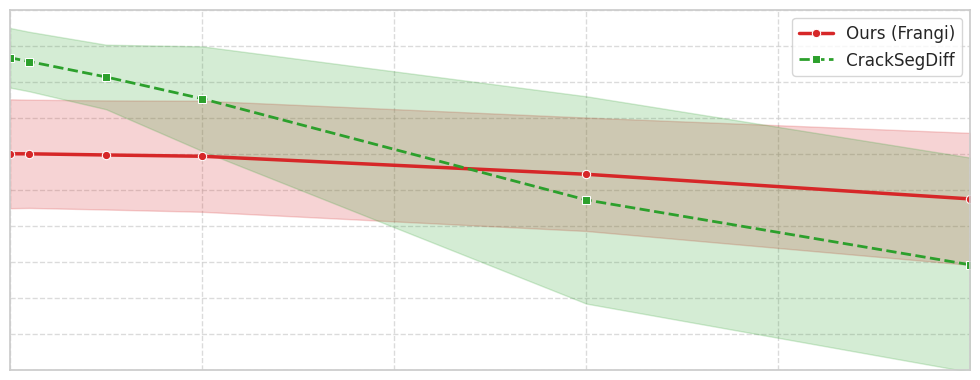
\includegraphics[width=20cm]{Jaccard_noisy.png}};
  \draw[-{Latex[length=4mm]},line width=0.6mm] (plot.south west)--(plot.north west);
  \draw[-{Latex[length=4mm]},line width=0.6mm] (plot.south west)--(plot.south east);
  \node[anchor=east] at (plot.north west) {100};
  \node[anchor=north east] at (plot.south west) {0};
  \node[anchor=north] at (plot.south east) {0.5};
  \node[anchor=south west] at (plot.north west) {Jaccard (\%)};
  \node[anchor=north,yshift=-.9cm] at (plot.south) {Synthetic noise level $s$};
\end{tikzpicture}
\par{\captiontext\colorline{red!80!black} Ours\quad\colorline{green!55!black} CrackSegDiff\quad Bands: standard deviation.}
\par\vspace{0.15cm}
\panel{0.245}{IntensityNoisy_1FIND.png}{Noisy intensity}
\hfill\panel{0.245}{RangeNoisy_1FIND.png}{Noisy range}
\hfill\panel{0.245}{ResultatNoisy_1FIND.png}{Our skeleton}
\par\RaggedRight{\captiontext $s=0.5$: multiplicative speckle on $I$, additive Gaussian noise on $R$.}
\end{block}
\end{posterpanel}

\begin{posterpanel}{\geologypanel}
\begin{block}{6. Geological domain shift~{\hypersetup{citecolor=white}\cite{zhang2025review}}}
\textbf{Vaches Noires.} Two Cerema UAV patches ($512\!\times\!512$).
\par\vspace{0.2cm}
\begin{minipage}[c]{0.78\linewidth}
\panel{0.482}{Test1_512_512_result.png}{Test1: 47\% / 50\%}
\hfill\panel{0.482}{Test2_512_512_result.png}{Test2: 29\% / 34\%}
\end{minipage}\hfill
\begin{minipage}[c]{0.19\linewidth}\RaggedRight
{\captiontext Jaccard:\par ours / U-Net.
\par\smallskip Transfer strategy~\cite{shi2023geocrack}; local U-Net trained on a separate image.}
\end{minipage}
\par{\captiontext\colorline{red} Ours\quad\colorline{blue} U-Net + transfer learning\quad\colorline{green} Ground truth}
\par{\smalltext U-Net: \textbf{about two days of expert annotation}; ours: none.}
\end{block}
\end{posterpanel}

\setlength{\leftcolumnheight}{\dimexpr\ht\fusepanel+\dp\fusepanel+\ht\linkpanel+\dp\linkpanel+\ht\centerpanel+\dp\centerpanel+\ht\palaispanel+\dp\palaispanel+3\posterblockgap\relax}
\setlength{\rightcolumnheight}{\dimexpr\ht\accuracypanel+\dp\accuracypanel+\ht\noisepanel+\dp\noisepanel+\ht\geologypanel+\dp\geologypanel+2\posterblockgap\relax}
\setlength{\maincolumnheight}{\leftcolumnheight}
\ifdim\rightcolumnheight>\maincolumnheight\setlength{\maincolumnheight}{\rightcolumnheight}\fi
\begin{columns}[T,onlytextwidth]
\begin{column}{0.488\textwidth}
\vbox to \maincolumnheight{\offinterlineskip
  \hbox{\usebox{\fusepanel}}\vfil
  \hbox{\usebox{\linkpanel}}\vfil
  \hbox{\usebox{\centerpanel}}\vfil
  \hbox{\usebox{\palaispanel}}\kern0pt}
\end{column}
\begin{column}{0.488\textwidth}
\vbox to \maincolumnheight{\offinterlineskip
  \hbox{\usebox{\accuracypanel}}\vfil
  \hbox{\usebox{\noisepanel}}\vfil
  \hbox{\usebox{\geologypanel}}\kern0pt}
\end{column}
\end{columns}
\vspace{\posterblockgap}

\begin{block}{Perspective: frozen SAM 2 + LoRA + Frangi hierarchy}
\begin{minipage}[c]{0.56\linewidth}
  \centering\tikzfigure{0.98\linewidth}{foundation-hierarchy}
\end{minipage}\hfill
\begin{minipage}[c]{0.415\linewidth}\RaggedRight
  \textbf{SAM 2~\cite{ravi2025sam2}: frozen pretrained weights.}\par
  \textbf{LoRA~\cite{hu2022lora} + one coefficient $\beta$: learned together.}
  \[A_H=\mathrm{softmax}(L+\beta B_H).\]
  {\smalltext $L$: visual scores; $B_H$: hierarchy bias.\par
  Merge heights describe connectivity~\cite{turaga2009malis}. We use them to bias attention,
  following Graphormer~\cite{ying2021graphormer}.
  CrackSAM~\cite{ge2024cracksam} motivates adaptation to cracks.\par
  \textbf{Aim: fewer breaks without more false links.}}
\end{minipage}
\end{block}

\begin{block}{References}
\begin{minipage}[c]{0.80\linewidth}
{\fontsize{18}{21}\selectfont\RaggedRight
\hypersetup{urlcolor=black}
\setlength{\columnsep}{0.8cm}\setlength{\multicolsep}{0pt}
\begin{multicols}{2}
\bibliographystyle{poster}
\bibliography{references}
\end{multicols}
\par\smallskip
\href{mailto:louis.hauseux@inria.fr}{louis.hauseux@inria.fr}\quad\textbullet\quad
\href{https://github.com/Ayana-Inria/Frangi-EUVIP}{github.com/Ayana-Inria/Frangi-EUVIP}}
\end{minipage}\hfill
\begin{minipage}[c]{0.17\linewidth}\centering
\href{https://github.com/Ayana-Inria/Frangi-EUVIP}{\XeTeXLinkBox{\textcolor{black}{%
\qrcode[height=6cm,hyperlink=false]{https://github.com/Ayana-Inria/Frangi-EUVIP}}}}
\par{\captiontext Code \& data}
\end{minipage}
\end{block}
\end{frame}
\end{document}
